\documentclass[mathserif ]{fancyslides} 
\usepackage[utf8]{inputenc}
\usepackage{times}
\usepackage{multicol}

%%% Beamer settings (do not change)
\usetheme{default} 
\setbeamertemplate{navigation symbols}{} %no navigation symbols
\setbeamercolor{structure}{fg=\yourowntexcol} 
\setbeamercolor{normal text}{fg=\yourowntexcol} 



%%%%%%%%%%%%%%%%%%%%%%%%%
%%% CUSTOMISATIONS %%%%%%
%%%%%%%%%%%%%%%%%%%%%%%%%

%%%% SLIDE ELEMENTS
\newcommand{\structureopacity}{0.75} %opacity for the structure elements (boxes and dots)
\newcommand{\strcolor}{blue} %elements colour (predefined blue; orange; green)

%%%% TEXT COLOUR
\newcommand{\yourowntexcol}{white}



%%%%%%%%%%%%%%%%%%%%%%%%%
%%% TITLE SLIDE DATA %%%%
%%%%%%%%%%%%%%%%%%%%%%%%%
\newcommand{\titlephrase}{Progressive Photon Mapping}
\newcommand{\authorname} {T. Hachisuka, S. Ogaki and H. Jensen}
\newcommand{\name}{Presented by: Garoe Dorta Perez}
\newcommand{\affil}{CM50245: Computer Animation and Games II}

\begin{document}

\startingslide %this generates titlepage from the data above

\fbckg{img/blank}
\begin{frame}
\misc{
	\begin{multicols}{2}
	\itemized{
	\item Rendering equation
	\item $L_o (x, \omega_o) = L_e(x, \omega_o) + \int_\Omega f(x, \omega_o, \omega_i) L_i(x, \omega_i) |cos \theta_i| d \omega_i$
	}
	\begin{figure}[b!]
	\includegraphics[scale=0.32]{img/Rendering_eq}
	\end{figure}
	\end{multicols}
}
\end{frame}


\fbckg{img/blank}
\begin{frame}
\itemized{
\item Photon mapping as an approximation
\item Two passes
	\begin{enumerate}
	\item Ray tracing in a photon map
	\item Photon rendering
	\end{enumerate}
\item $L_r (x, \omega_o) \approx \sum_{p=1}^N \frac{f(x, \omega_o, \omega_i) \phi_p (x_p, \omega_i)}{\pi r^2} $
}
\end{frame}

\fbckg{img/blank}
\begin{frame}
\itemized{
\item Ray tracing pass 1
	\begin{multicols}{2}
	\itemized{
	\item Building photon map
	\item Ray tracing to find visible surfaces
	\item Each ray includes all specular bounces
	\item Stop when non-specular surface is found
	}
	\begin{figure}[b!]
	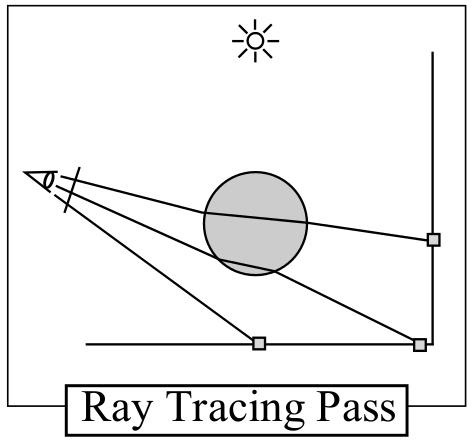
\includegraphics[scale=0.35]{img/ray_tracing}
	\end{figure}
	\end{multicols}
}
\end{frame}

\fbckg{img/blank}
\begin{frame}
\itemized{
\item Ray tracing pass 2
	\begin{multicols}{2}
	\itemized{
	\item Struct hitPoint
	\begin{enumerate}
		\item[$x$] hit position
		\item[i,j] pixel location
		\item[$R$] current radius
		\item[$N$] acum photon count
		\item[$\tau$] acum reflected flux
	\end{enumerate}
	}
	\begin{figure}[b!]
	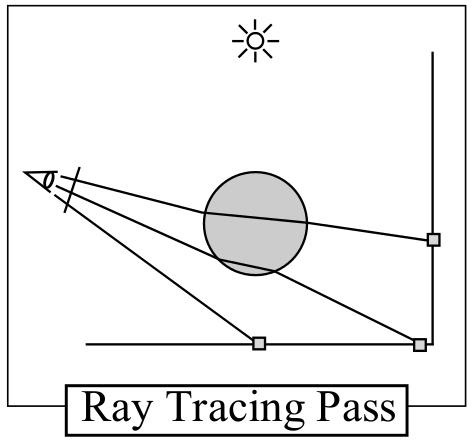
\includegraphics[scale=0.35]{img/ray_tracing}
	\end{figure}
	\end{multicols}
}
\end{frame}

\fbckg{img/blank}
\begin{frame}
\itemized{
\item Photon tracing pass
	\begin{multicols}{2}
	\itemized{
	\item Accumulate photon flux in hit points
	\item New photons improve the quality
	\item $d(x) = \frac{n}{\pi r^2}, ~ d'(x) = \frac{n'}{\pi r^2} $
	}
	\begin{figure}[b!]
	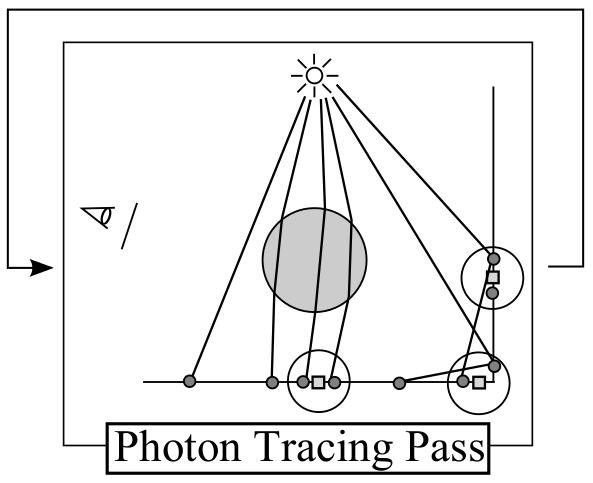
\includegraphics[scale=0.3]{img/photon_tracing}
	\end{figure}
	\end{multicols}
}
\end{frame}

\fbckg{img/blank}
\begin{frame}
\itemized{
\item Radius reduction
	\itemized{
		\item Radius reduces with each pass to increase quality
		\item There has to be a gain in total number of photons
		\item Keep fraction of new photons $\hat{N}(x) = N(x) + \alpha M(x)$
		\item New radius $\hat{R}(x) = R(x) \left(\frac{N(x) + \alpha M(x)}{N(x) + M(x)}  \right)^{\frac{1}{2}}$
	}
}
\end{frame}

\fbckg{img/blank}
\begin{frame}
\itemized{
\item Flux correction
	\itemized{
		\item Reduced radius = incorrect accumulated flux
		\item $\tau_N(x, \omega_o) = \sum_{p=1}^{N(x)} f(x, \omega_o, \omega_i) \phi'_p(x_p, \omega_i) $
		\item $\tau_{\hat{N}}(x, \omega_o) = \left( \tau_{N}(x, \omega_o) + \tau_{M}(x, \omega_o) \right) \frac{N(x) + \alpha M(x)}{N(x) + M(x)}$
	}
}
\end{frame}

\fbckg{img/blank}
\begin{frame}
\itemized{
\item Radiance evaluation
	\itemized{
		\item Sum the contribution of all photons in the hit point
		\item $L(x, \omega_o) = \frac{\tau(x, \omega_o)}{\pi R(x)^2 N_{em}} $
	}
}
\end{frame}

\usebackgroundtemplate{%
  \vbox to \paperheight{\vfil\hbox to \paperwidth{\hfil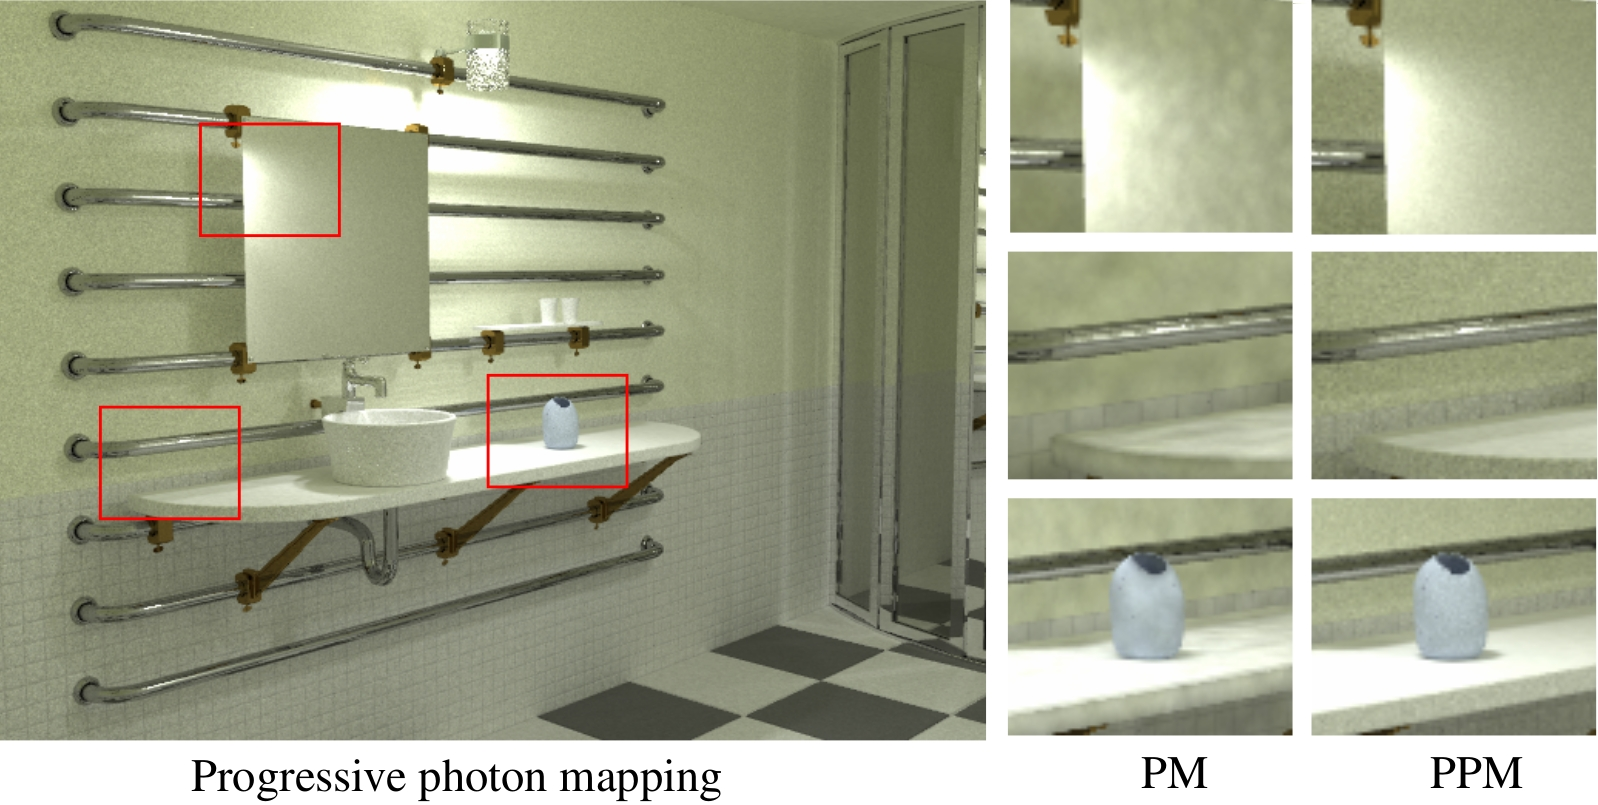
\includegraphics[width=\paperwidth]{img/bath_ppm}\hfil}\vfil}
}
\begin{frame}
\end{frame}

\usebackgroundtemplate{%
  \vbox to \paperheight{\vfil\hbox to \paperwidth{\hfil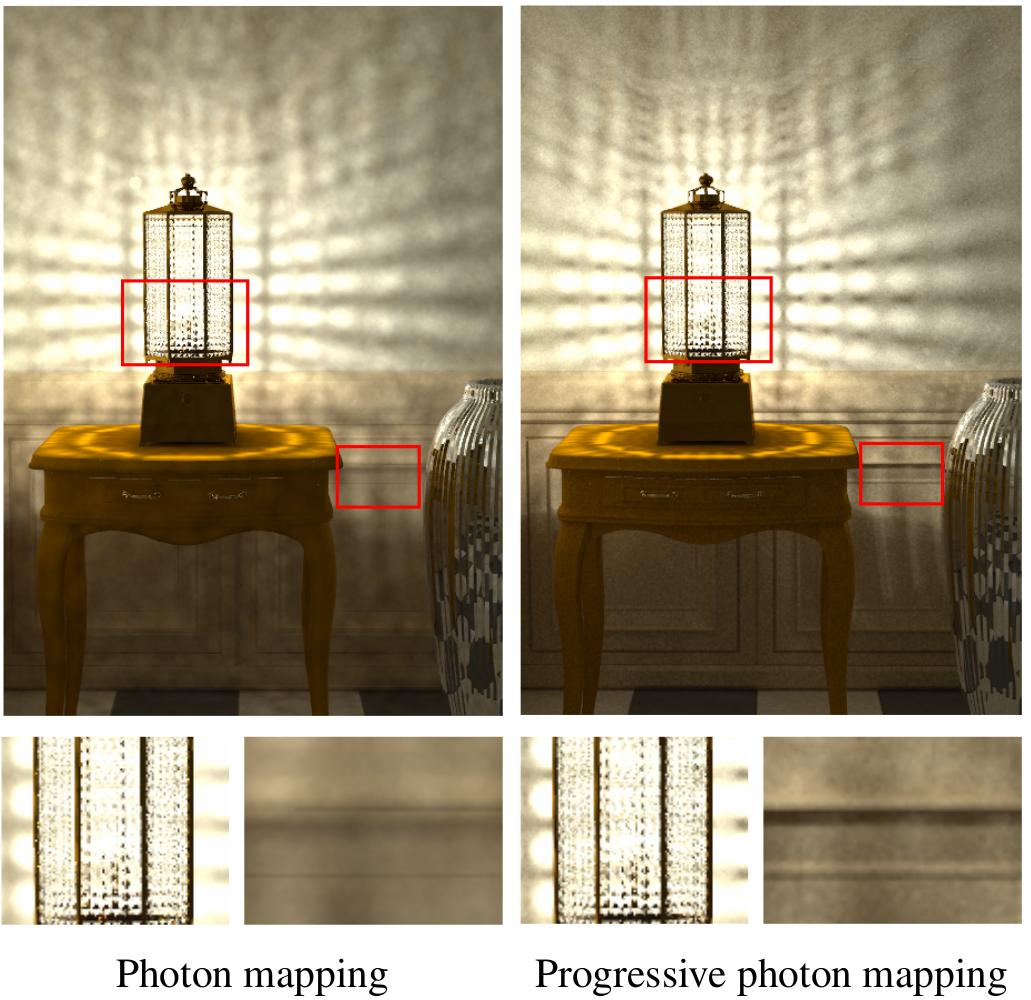
\includegraphics[height=\paperheight]{img/lamp_ppm}\hfil}\vfil}
}
\begin{frame}
\end{frame}

\fbckg{img/blank}
\begin{frame}
\itemized{
\item Possible improvements
	\itemized{
		\item Locally adaptive
		\item Optimal number of total photons
		\item Optimal direction to shoot photons
		\item Optimal photon intensity
	}
}
\end{frame}

\fbckg{img/blank}
\begin{frame}
\misc{ \begin{center}
Questions?
\end{center}  }
\end{frame}

\end{document}